\documentclass{article}
\usepackage[utf8]{inputenc}

\title{WydenArea1CalculoNumerico}
%\author{Heleno Cardoso}
\author{
  Heleno Cardoso da S. Filho\thanks{PPGCOMP UNIFACS - Mestre em Sistemas e Computação -- PGCOMP UFBA [Aluno Especial no Doutorado em Ciência da Computação].} \\
  Departamento de Engenharia\\
  Wyden Faculdade Área 1\\
  Brasil - Adtalem Global Education\\
  \texttt{helenocardosofilho@gmail.com} \\
  %% examples of more authors
  %% \And
  %% Coauthor \\
  %% Affiliation \\
  %% Address \\
  %% \texttt{email} \\
  %% \AND \\
}
\date{August 2018}

\usepackage{natbib}
\usepackage{graphicx}

\begin{document}

\maketitle

\section{Disciplina Cálculo Numérico - Wyden Área 1}
-- ZERO DE FUNÇÃO - BISSECÇÃO
https://www.youtube.com/watch?v=AXt9dq_AjOo

-- Complemento de 1 e 2 - História
https://medium.com/@jeanfelipemartinsdacosta/sinal-magnitude-bit-de-sinal-complemento-de-1-e-complemento-de-2-a1d32045ab18

https://www.ensinoeinformacao.com

Cálculo da Estimativa de Iterações - Métodos Zeros de Funções

n > ( log (b - a) - log ϵ ) / log 2

Ex.: [0.5;1]; ϵ < 0.05

n > ( log(1-0.05) - log 0.005 ) log 2

n > 3.32 => n > 4 iterações

Ex. Ponto Fixo
https://www.youtube.com/watch?v=PFwKBhluGSE

f(x) = x^2 + x - 6 (Gera três equações) analisar a convergência



Quadratura Gaussiana - Métodos Numéricos
https://slideplayer.com.br/slide/285692/

As principais fontes de erros são as seguintes:

erros nos dados de entrada;
erros no estabelecimento do modelo matemático;
erros de arredondamento durante a computação;
erros de truncamento, e
erros humanos e de máquinas.
***************************************


Introduzir os fundamentos dos métodos numéricos básicos utilizados na solução (tipicamente aproximada) de problemas matemáticos, algébricos e diferenciais, de caráter linear ou não linear, que aparecem comumente nas ciências puras e aplicadas e também nas engenharias.

Podemos dividir a Matemática em duas partes, o cálculo numérico e o cálculo algébrico. O cálculo numérico envolve as operações da adição, subtração, multiplicação, divisão, potenciação e radiciação, envolvendo os números reais. Os cálculos envolvendo frações, também são abordados e explorados de forma complexa. 
O calculo algébrico está diretamente ligado às expressões algébricas, envolvendo equações, inequações e sistemas de equações. Nele, todos os fundamentos fixados no cálculo numérico são utilizados. 

\section{Conclusão}

Cálculo Numérico: O Cálculo Numérico tem por objetivo estudar esquemas numéricos (algoritmos numéricos) para resolução de problemas que podem ser representados por um Modelo Matemático. Um esquema é eficiente quando este apresenta soluções dentro de uma precisão desejada com custo computacional (tempo de execução + memória) baixo. Os esquemas numéricos nos fornecem aproximações para o que seria a solução exata do problema. Os erros cometidos nesta aproximação são decorrentes da discretização do problema, ou seja, passar do Modelo Matemático para o esquema numérico, e da forma como as máquinas representam os dados numéricos.

Esperando não sermos prolixos, mais resumidamente, Cálculo Numéricos constitui-se de: Um Conjunto de Ferramentas ou Métodos usados para se obter a Solução de problemas Matemáticos de Forma Aproximada. Esses Métodos se aplicam principalmente a Problemas que não apresentam uma Solução Exata obtida Analiticamente, portanto precisam ser Resolvidos Numericamente.

\begin{figure}[h!]
\centering
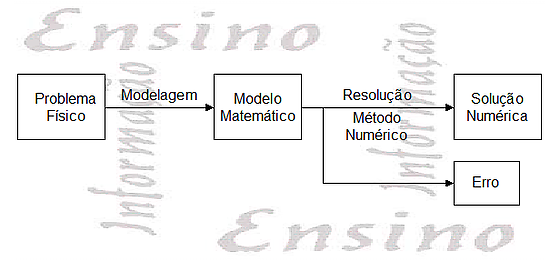
\includegraphics[scale=0.85]{SolucaoCalculoNumerico}
\caption{Cálculo Numérico}
\label{fig:SolucaoCalculoNumerico}
\end{figure}

Modelagem: Fase de obtenção de um Modelo Matemático que Descreva o Comportamento do Sistema Físico em questão. Os Erros na Fase de Modelagem são de início atribuídos pela SIMPLIFICAÇÃO do Problema Físico (da Realidade)!

Resolução: Fase de obtenção da Solução do Modelo Matemático através da Aplicação de Métodos Numéricos por meio de Instrumentos de Cálculo (Calculadoras, Computadores, Instrumentos de Medida, e etc...).

\end{document}
